\documentclass{article}
\usepackage[margin=1in]{geometry}

\usepackage{amsmath}          % <- gives you bmatrix, pmatrix, etc.
\usepackage{tikz}
\usetikzlibrary{positioning,calc,arrows.meta}
\usepackage{pgfplots}
\pgfplotsset{compat=1.18}
\usepgfplotslibrary{fillbetween}

\renewcommand*{\arraystretch}{1.25}
\newcommand{\relu}{\mathrm{ReLU}}
\newcommand{\id}{\mathrm{Id}}

% --- styles and reusable macro (unchanged) ---
\tikzset{
  neuron/.style   = {circle,draw,minimum width=3cm},
  vect/.style     = {inner sep=0pt},
  actlabel/.style = {inner sep=0pt, font=\scriptsize},
  >={Stealth[scale=2]}
}
\newcommand{\DrawNeuron}[5]{%
  % draws the circle (neuron)
  \node[neuron] (#1) at #2 {};
  % displays input vector (left half)
  \node[vect]   at ($(#1.center)+(-0.5,0)$) {#4};
  % draws the vertical line through neuron (activation boundary)
  \draw         ($(#1.center)+(0.2,1.2cm)$)--($(#1.center)+(0.2,-1.2cm)$);
  % displays activation function label (right half)
  \node[actlabel]at ($(#1.center)+(0.9,0)$) {#5};
  % displays layer label (top)
  \node[above=0pt of #1] {#3};
}

\begin{document}

\section{Logical AND}
\[
  \{0,1\}^2 \to \{0,1\}
\]

\begin{align*}
  U_0 &= \id\left(
    \begin{bmatrix}
      x^{(0)}_{1} \\
      x^{(0)}_{2}
  \end{bmatrix}\right) \\
  U_1 &=\relu\left(
    \begin{bmatrix}
      \id\left( x^{(0)}_{1} \right) + \id\left( x^{(0)}_{2} \right) - 1
    \end{bmatrix}
  \right)
\end{align*}

\begin{center}
  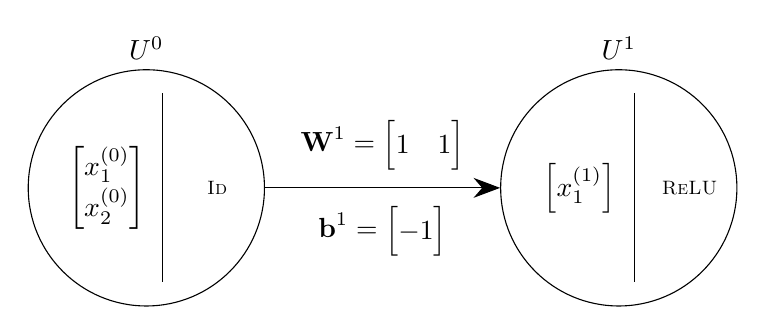
\begin{tikzpicture}
    \DrawNeuron{u0}{(0,0)}
    {$U^{0}$}
    {$ % TODO: big or little x?
      \begin{bmatrix}x^{(0)}_{1}\\x^{(0)}_{2}
    \end{bmatrix}$}
    {\textsc{Id}}

    \DrawNeuron{u1}{(6,0)}
    {$U^{1}$}
    {$
      \begin{bmatrix}x^{(1)}_{1}
    \end{bmatrix}$}
    {\textsc{ReLU}}

    \draw[->] (u0) -- (u1);

    \path let \p1 = ($(u0)!0.5!(u1)$) in
    node[above=3pt] at (\p1) {$\textbf{W}^{1}=
      \begin{bmatrix}1&1
    \end{bmatrix}$}
    node[below=3pt] at (\p1) {$\textbf{b}^{1}=
      \begin{bmatrix}-1
    \end{bmatrix}$};
  \end{tikzpicture}
\end{center}

\section{Logical NOT}

\begin{align*}
  U_0 &= \id\left(
    \begin{bmatrix}
      x^{(0)}_{1}
  \end{bmatrix}\right) \\
  U_1 &= \id\left(
    \begin{bmatrix}
      - \id\left( x^{(0)}_{1} \right) + 1
  \end{bmatrix}\right)
\end{align*}

\begin{center}
  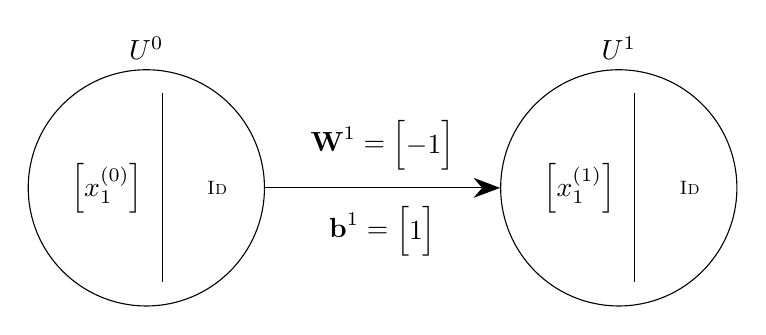
\begin{tikzpicture}
    \DrawNeuron{u0}{(0,0)}
    {$U^{0}$}
    {$
      \begin{bmatrix}x^{(0)}_{1}
    \end{bmatrix}$}
    {\textsc{Id}}

    \DrawNeuron{u1}{(6,0)}
    {$U^{1}$}
    {$
      \begin{bmatrix}x^{(1)}_{1}
    \end{bmatrix}$}
    {\textsc{Id}}

    \draw[->] (u0) -- (u1);

    \path let \p1 = ($(u0)!0.5!(u1)$) in
    node[above=3pt] at (\p1) {$\textbf{W}^{1}=
      \begin{bmatrix}-1
    \end{bmatrix}$}
    node[below=3pt] at (\p1) {$\textbf{b}^{1}=
      \begin{bmatrix}1
    \end{bmatrix}$};
  \end{tikzpicture}
\end{center}

\section{Logical OR}

\[
  \{0,1\}^2 \to \{0,1\}
\]

Let $S$ be the sum of the inputs, which is $x^{(0)}_1 + x^{(0)}_2$.
We output whether $S>0$ by the taking the ReLU
of $S$ and $S-1$. If $S\le 0$, then $0-0=0$. If $S>0$, then $S-(S-1)=1$.

\begin{align*}
  U_0 &= \id\left(
    \begin{bmatrix}
      x^{(0)}_{1} \\
      x^{(0)}_{2}
  \end{bmatrix}\right) \\
  U_1 &= \relu\left(
    \begin{bmatrix}
      \id\left( x^{(0)}_{1} + x^{(0)}_{2} \right) \\
      \id\left( x^{(0)}_{1} + x^{(0)}_{2} \right) - 1
  \end{bmatrix}\right) \\
  U_2 &= \id\left(
    \begin{bmatrix}
      \relu\left( \id\left( x^{(0)}_{1} + x^{(0)}_{2} \right) \right)
      - \relu\left( \id\left( x^{(0)}_{1} + x^{(0)}_{2} \right) - 1 \right)
    \end{bmatrix}
  \right)
\end{align*}

\begin{center}
  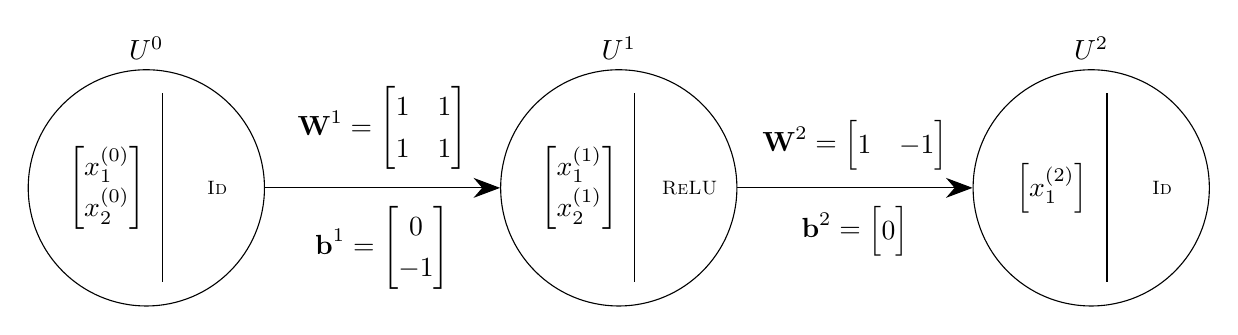
\begin{tikzpicture}
    \DrawNeuron{u0}{(0,0)}
    {$U^{0}$}
    {$
      \begin{bmatrix}x^{(0)}_{1}\\x^{(0)}_{2}
    \end{bmatrix}$}
    {\textsc{Id}}

    \DrawNeuron{u1}{(6,0)}
    {$U^{1}$}
    {$
      \begin{bmatrix}x^{(1)}_{1}\\x^{(1)}_{2}
    \end{bmatrix}$}
    {\textsc{ReLU}}

    \draw[->] (u0) -- (u1);

    % weights and biases 1
    \path let \p1 = ($(u0)!0.5!(u1)$) in
    node[above=3pt] at (\p1) {$\textbf{W}^{1}=
      \begin{bmatrix}1&1\\1&1
    \end{bmatrix}$}
    node[below=3pt] at (\p1) {$\textbf{b}^{1}=
      \begin{bmatrix}0\\-1
    \end{bmatrix}$};

    \DrawNeuron{u2}{(12,0)}
    {$U^{2}$}
    {$
      \begin{bmatrix}x^{(2)}_{1}
    \end{bmatrix}$}
    {\textsc{Id}}

    % weights and biases 2
    \draw[->] (u1) -- (u2);
    \path let \p1 = ($(u1)!0.5!(u2)$) in
    node[above=3pt] at (\p1) {$\textbf{W}^{2}=
      \begin{bmatrix}1&-1
    \end{bmatrix}$}
    node[below=3pt] at (\p1) {$\textbf{b}^{2}=
      \begin{bmatrix}0
    \end{bmatrix}$};
  \end{tikzpicture}
\end{center}

\section{Logical XOR}

\[
  \{0,1\}^2 \to \{0,1\}
\] \marginpar{\raggedright TODO: what if more than 2 inputs?}

We can think of binary XOR as returning 1 if the inputs are
different, and 0 if they are the same. For the second case, we can
take advantage of the fact that the difference between two identical
numbers is 0. Thus, we take the ReLU of the difference between the
two inputs in both directions, that is, $\relu\left( x^{(0)}_1 -
x^{(0)}_2 \right)$ and $\relu\left( x^{(0)}_2 - x^{(0)}_1 \right)$.
If the inputs are the same, $0+0=0$. If the inputs are different, the
difference in one direction is 1 and the other is -1 rectified to 0,
resulting in 1.

\begin{align*}
  U_0 &= \id\left(
    \begin{bmatrix}
      x^{(0)}_{1} \\
      x^{(0)}_{2}
  \end{bmatrix}\right) \\
  U_1 &= \relu\left(
    \begin{bmatrix}
      \id\left( x^{(0)}_{1} - x^{(0)}_{2} \right) \\
      \id\left( x^{(0)}_{2} - x^{(0)}_{1} \right)
  \end{bmatrix}\right) \\
  U_2 &= \id\left(
    \begin{bmatrix}
      \relu\left( \id\left( x^{(0)}_{1} - x^{(0)}_{2} \right) \right)
      + \relu\left( \id\left( x^{(0)}_{2} - x^{(0)}_{1} \right) \right)
    \end{bmatrix}
  \right)
\end{align*}

\begin{center}
  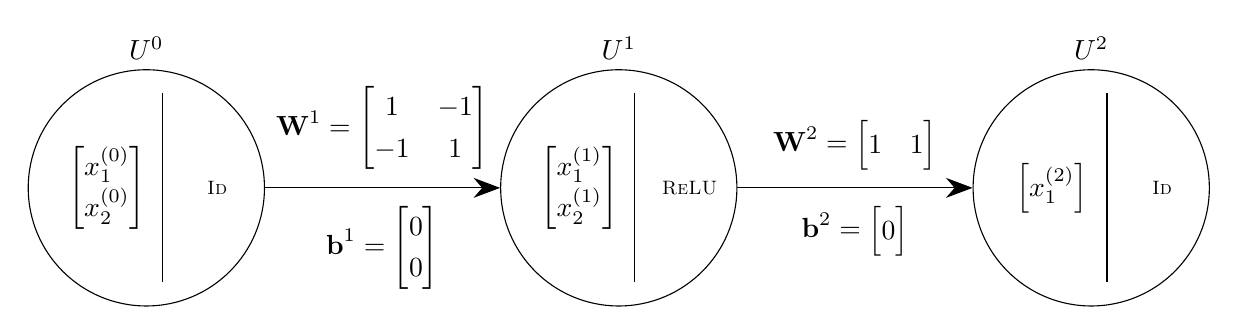
\begin{tikzpicture}
    \DrawNeuron{u0}{(0,0)}
    {$U^{0}$}
    {$
      \begin{bmatrix}x^{(0)}_{1}\\x^{(0)}_{2}
    \end{bmatrix}$}
    {\textsc{Id}}

    \DrawNeuron{u1}{(6,0)}
    {$U^{1}$}
    {$
      \begin{bmatrix}x^{(1)}_{1}\\x^{(1)}_{2}
    \end{bmatrix}$}
    {\textsc{ReLU}}

    \draw[->] (u0) -- (u1);

    % weights and biases 1
    \path let \p1 = ($(u0)!0.5!(u1)$) in
    node[above=3pt] at (\p1) {$\textbf{W}^{1}=
      \begin{bmatrix}1&-1\\-1&1
    \end{bmatrix}$}
    node[below=3pt] at (\p1) {$\textbf{b}^{1}=
      \begin{bmatrix}0\\0
    \end{bmatrix}$};

    \DrawNeuron{u2}{(12,0)}
    {$U^{2}$}
    {$
      \begin{bmatrix}x^{(2)}_{1}
    \end{bmatrix}$}
    {\textsc{Id}}

    % weights and biases 2
    \draw[->] (u1) -- (u2);
    \path let \p1 = ($(u1)!0.5!(u2)$) in
    node[above=3pt] at (\p1) {$\textbf{W}^{2}=
      \begin{bmatrix}1&1
    \end{bmatrix}$}
    node[below=3pt] at (\p1) {$\textbf{b}^{2}=
      \begin{bmatrix}0
    \end{bmatrix}$};
  \end{tikzpicture}
\end{center}

\section{Logistic Regression}

\begin{align*}
  U_0 &= \id\left(
    \begin{bmatrix}
      x^{(0)}_{1} \\
      x^{(0)}_{2}
  \end{bmatrix}\right) \\
  U_1 &= \sigma\left(
    \begin{bmatrix}
      a\cdot\id\left( x^{(0)}_{1} \right) +
      b\cdot\id\left( x^{(0)}_{2} \right) +
      c\cdot\id\left( x^{(0)}_{3} \right) + d
    \end{bmatrix}
  \right)
\end{align*}

\begin{center}
  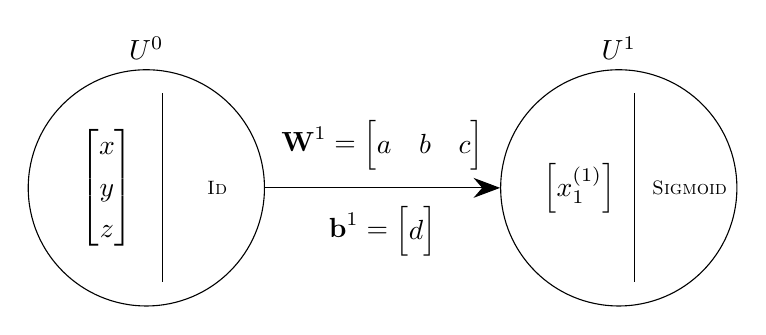
\begin{tikzpicture}
    \DrawNeuron{u0}{(0,0)}
    {$U^{0}$}
    {$
      \begin{bmatrix}x\\y\\z
    \end{bmatrix}$}
    {\textsc{Id}}

    \DrawNeuron{u1}{(6,0)}
    {$U^{1}$}
    {$
      \begin{bmatrix}x^{(1)}_{1}
    \end{bmatrix}$}
    {\textsc{Sigmoid}}

    \draw[->] (u0) -- (u1);

    \path let \p1 = ($(u0)!0.5!(u1)$) in
    node[above=3pt] at (\p1) {$\textbf{W}^{1}=
      \begin{bmatrix}a&b&c
    \end{bmatrix}$}
    node[below=3pt] at (\p1) {$\textbf{b}^{1}=
      \begin{bmatrix}d
    \end{bmatrix}$};
  \end{tikzpicture}
\end{center}

\section{Two-Variable Function}

\begin{center}
  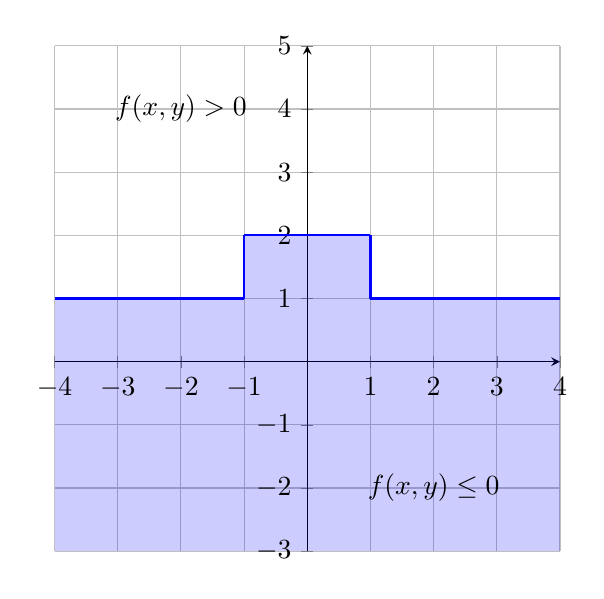
\begin{tikzpicture}
    \begin{axis}[
        axis equal,
        axis lines=middle,
        grid=major,
        xmin=-4, xmax=4, ymin=-3, ymax=5,
        xtick={-4,-3,-2,-1,0,1,2,3,4},
        ytick={-3,-2,-1,0,1,2,3,4,5},
        width=8cm, height=8cm
      ]
      \addplot[blue, thick] coordinates {(-1,1) (-1,2)};
      \addplot[blue, thick] coordinates {(1,1) (1,2)};

      % Left region: x ∈ [-4,-1], y ∈ [-3,1]
      \addplot[blue, thick, name path=top1, domain=-4:-1, samples=2] {1};
      \addplot[name path=bot1, domain=-4:-1, draw=none, samples=2] {-3};
      \addplot[fill=blue, fill opacity=0.2] fill between[of=top1 and bot1];

      % Right region: x ∈ [1,4], y ∈ [-3,1]
      \addplot[blue, thick, name path=top2, domain=1:4, samples=2] {1};
      \addplot[name path=bot2, domain=1:4, draw=none, samples=2] {-3};
      \addplot[fill=blue, fill opacity=0.2] fill between[of=top2 and bot2];

      % Middle region: x ∈ [-1,1], y ∈ [-3,2]
      \addplot[blue, thick, name path=top3, domain=-1:1, samples=2] {2};
      \addplot[name path=bot3, domain=-1:1, draw=none, samples=2] {-3};
      \addplot[fill=blue, fill opacity=0.2] fill between[of=top3 and bot3];

      % Notate function outputs at each region
      \node at (axis cs:-2,4) {$f(x,y) > 0$};
      \node at (axis cs:2,-2) {$f(x,y) \le 0$};
    \end{axis}
  \end{tikzpicture}
\end{center}

\end{document}
